\documentclass[conference]{IEEEtran}
\IEEEoverridecommandlockouts
% The preceding line is only needed to identify funding in the first footnote. If that is unneeded, please comment it out.
\usepackage[square]{natbib}
\setcitestyle{numbers}
\usepackage{amsmath,amssymb,amsfonts}
\usepackage{algorithmic}
\usepackage{graphicx}
\usepackage{textcomp}
\usepackage{xcolor}
\def\BibTeX{{\rm B\kern-.05em{\sc i\kern-.025em b}\kern-.08em
    T\kern-.1667em\lower.7ex\hbox{E}\kern-.125emX}}
\begin{document}

\title{Using CNN for letter recognition in images}

\author{\IEEEauthorblockN{Daniel Aaron Salwerowicz}
\IEEEauthorblockA{\textit{Institutt for datateknologi og beregningsorienterte ingeniørfag} \\
\textit{Arctic University of Norway, Narvik}\\
Narvik, Norway \\
dsa014@post.uit.no}
}

\maketitle

\begin{abstract}
In this report I describe my research related to developing CNN (Convolutional Neural Network) from scratch and then finding the best parameters to train it in recognizing letters in images. It shows how image is processed in between layers using my own implementation of them and then it shows what are the best parameters to use in such a network to develop best working model.
\end{abstract}

\begin{IEEEkeywords}
CNN, kernel, stride, letter recognition, object recognition, cifar10
\end{IEEEkeywords}

\section{Introduction}
This research project revolved around finding the best parameters for learning a neural network to recognize letters in images. Parameters that I looked on were the pooling size, kernel and stride for convolutional layer, and dropout rate in between layers.

\section{Problem specification}
\section{Methods applied}
\section{Results}
\section{Discussion}

%\begin{figure}[htbp]
%\centerline{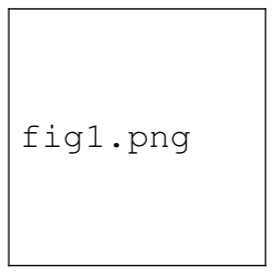
\includegraphics{fig1.png}}
%\caption{Example of a figure caption.}
%\label{fig}
%\end{figure}

\section*{Acknowledgments}

\bibliographystyle{apalike}
\bibliography{Bibliography}

\end{document}
